\documentclass[12pt]{article}

\usepackage[T1]{fontenc}
\usepackage[utf8]{inputenc}
\usepackage{lmodern}

\usepackage[ngerman, english]{babel} 

\usepackage{csquotes}

\usepackage{amsmath}

\usepackage{siunitx}
\sisetup{locale=US}
\sisetup{separate-uncertainty=true}

\usepackage{color}

\usepackage{geometry}
\geometry{a4paper, top=15mm, left=20mm, right=20mm, bottom=30mm, headsep=10mm, footskip=20mm}

\usepackage[backend=biber, style=numeric]{biblatex}
\addbibresource{bib/references.bib}

\usepackage{graphicx}

\setlength{\columnsep}{10mm} % set length of the gap between two columns
\setlength{\parindent}{0mm} % set length of indentation of a paragraph
\setlength{\parskip}{2mm} % set length of the gap between two paragraphs

\usepackage{adjustbox} % used for \adjustbox

\usepackage{units} % used for \nicefrac

\usepackage{hyperref} % automatically create clickable links

\usepackage{multicol} % used for \begin{multicols} to create a column layout

\usepackage{caption} % used for \captionsetup and \captionof

\usepackage{sectsty} % used for \allsectionsfont
\allsectionsfont{\sffamily}

\usepackage{framed} % used for \begin{snugshade*}
\definecolor{shadecolor}{RGB}{230, 230, 230} % set background color for \begin{snugshade*}

\usepackage{booktabs} % used for \toprule, \midrule and \bottomrule with tables

\makeatletter
\newcommand*{\header}[1]{\gdef\@header{#1}}
\def\@maketitle{
    \begin{flushleft}
    \Large
    \textsf{\@header}
    \par
    \vskip 0mm
    \LARGE
    \textsf{\textbf{\@title}}
    \par
    \vskip 2mm
    \large
    \textsf{{\@author} | durchgeführt in der Woche vom \@date}
    \end{flushleft}
    \vskip 2mm
    }
\makeatother
 % import custom \maketitle command
\header{Protokoll Fortgeschrittenen-Praktikum}
\title{F83 Koinzidenzspektrometer}
\author{Vorname Name, Vorname Name}
\date{01.01.1970}

\begin{document}

\maketitle

\section{Introduction}
% Versuch geht um radioaktiven Zerfall und die Untersuchung der entstehenden Gammaquanten mithilfe Szintillationsspektroskopie
This article is about our experiment on radioactive decay of different radioactive elements and the study on the subsequently appearing $\gamma$ rays with the aid of scintillation spectroscopy.
%
\subsection{Radioactive decay}
% Atomkerne mehrere Stadien außer stabil.
Besides the stable state, there are various conditions an atomic nucleus can exist with.
% Falls instabil, radioaktive Strahlung.
If its state is unstable, the nucleus decays and emits radiation in the process.
% Mehrere Möglichkeiten für nach Zerfall: für uns wichtig beta und Übergänge zwischen den Anregungsstadien.
This is called radioactive decay and among others it may result in multiple modes of $\beta$ decay as well as transitions between different excitation states of the same nucleus.
%
\subsection{Modes of $\beta$ decay}
% beta-
The process of a decaying neutron resulting in the emission of an electron and an electron antineutrino is called \textbf{$\beta^{-}$ decay}.
A newly formed proton remains with the nucleus.
% beta+
The related process would be \textbf{$\beta^{+}$ decay} during which the nucleus obtains a neutron and emits a positron and an electron neutrino following a decaying proton.
% Electron Capture
Another mode is \textbf{electron capture} (EC) which takes place if an orbiting electron is being captured by a proton of the nucleus. Consequently, an electron neutrino is being emitted and the nucleus remains in an excited state.
%
\subsection{Transitions between excitation states}
% Isomeric transition
A $\gamma$ ray is emitted if an orbital electron of an excited nucleus wanders to a lower energy state.
This is called \textbf{isomeric transition} (IT).
% Internal conversion
The process of \textbf{internal conversion} (IC) denotes the transfer of energy of an excited nucleus onto one of its shell's electrons which results in the ejection of said electron from the atom.
%
\subsection{Interaction of $\gamma$ rays with matter}
% Falls gamma auf Materie trifft gibt es Wechselwirkung. Kann ausgenutzt werden für Spektrometer.
If $\gamma$ rays encounter matter, there are various possibilities of interaction. These interactions can be detected and used to build spectrometers.
%
\subsubsection{Photo effect}
% Photoeffekt tritt auf wenn Photonen passender Energie auf Materie treffen und somit Elektronen rausschlagen
The photo effect occurs when photons of adequate energy strike matter which results in emission of electrons.
% Gamma überträgt seine gesamte Energie auf ein Elektron und schlägt es damit aus der Hülle eines Atoms heraus
A $\gamma$ quantum transfers its complete energy onto one electron and thereby liberates it from the atom.
%
\subsubsection{Compton scattering}
% Stoß von gamma mit Elektron heißt Compton
Inelastic scattering of a $\gamma$ quantum with an electron is called Compton scattering.
% Photon verliert Energie
The photon transfers energy onto the electron which consequently increases the photon's wavelength.
% Energie hängt vom Winkel ab
The amount of energy which is transferred onto the electron depends on the scattering angle $\theta$:
\begin{align}
    \label{eq:PhotonNachStoss}
    \begin{split}
        {E_{\gamma}}'(\theta) &= E_{\gamma} - \frac{E_{\gamma}}{1 + \left ( 1 - \cos(\theta) \right ) \frac{E_{\gamma}}{m_{\text{e}} c^2}}
    \end{split}
    \\
    \label{eq:ElektronNachStoss}
    \begin{split}
        E_{\text{e}}(\theta) &= E_{\gamma} - {E_{\gamma}}'(\theta)
    \end{split}
\end{align}
where $E_{\gamma}$ and ${E_{\gamma}}'$ are the energies of the photon before and after the collision, $E_{\text{e}}$ is the energy of the electron after the collision, $m_{\text{e}}$ is the mass of the electron and $c$ is the speed of light. \cite{AnleitungZusatz2}
%
\subsubsection{Pair production}
% Falls Energie von gamma größer als Ruheenergie dann Paarbildung möglich was das Photon zu Elektron Positron Paar macht
If the energy of the $\gamma$ quantum exceeds \SI{1022}{\kilo\electronvolt}, which is the rest mass of an electron-positron pair, pair production may take place and the photon is converted into an electron-positron pair.
The involved nucleus ensures conservation of momentum.
\cite{AnleitungZusatz1}
%
\subsection{Scintillators}
% Angeregter Szintillator emittiert sichtbares oder UV-Licht
When a scintillator is being excited with high energy photons, it emits light of visible or ultraviolet range.
% Wir nutzen anorganischen Szintillator weil besser laut Aussagen in Anleitung
Even though organic scintillators exist as well, anorganic scintillators are better suited to detect $\gamma$ rays due to their higher atomic number and density. \cite{Anleitung}
%
\subsection{Scintillation spectrometer}
% Auftreffende gamma geben Energie an Elektronen
Impacting $\gamma$ rays transfer their energy onto electrons of the scintillator material as described above.
% Diese Elektronen gehen ins Leitungsband oder bilden Exziton
In turn, these electrons leave the valence band for the conduction band while creating an electron hole as well or - in case of an insufficient amount of transferred energy - form an exciton.
% Danach diffundieren die Energieträger zu den angelegten Fehlstellen
Either way, electrons, electron holes and excitons diffuse through the semiconductor until they encounter one of the inhomogeneities which have actively been created by doping.
% Dort existieren Energielevel zwischen Valenz- und Leitungsband sodass die Energieträger dort Energie abgeben können, was Photonen erzeugt
They act as an emission center by creating energy levels between the levels of the conduction and valence band - therefore promoting the energy carriers to dispose their energy which results in generated photons.
% Die Lichtblitze werden mit Photomultiplier detektiert
These flashes of light can then be detected with a photomultiplier tube.

\section{Procedures}
%
\subsection{Setup and initial measurements}
%
In the following text, the counter on the left (labeled "1") of our setup will be called "counter 1" and the one on the right (labeled "2") "counter 2".
%
\par
%
We set the voltage for counter 1 to $\SI{540 \pm 2}{\volt}$ and for counter 2 to $\SI{490 \pm 2}{\volt}$.
The cables which carry the signals from the spectroscopes are plugged directly into the oscilloscope.
We insert the $^{60}\text{Co}$ sample (labeled "NN258") into the detector chamber and close the sliding door.
On the oscilloscope screen, pulses of different height and length can be seen.
Exemplary screenshots for a quantitative analysis are listed in the appendix:
Figure \ref{fig:OsciSignal1} shows a signal from detector 1 with a pulse height of $\SI{50 \pm 5}{\milli\volt}$ and a pulse length of $\SI{100 \pm 10}{\micro\second}$.
Detector 2 is shown in figure \ref{fig:OsciSignal2} with two signals with a pulse height of $\SI{240 \pm 20}{\milli\volt}$ and a pulse length of $\SI{50 \pm 5}{\micro\second}$ or a pulse height of $\SI{50 \pm 5}{\milli\volt}$ and a pulse length of $\SI{30 \pm 5}{\micro\second}$, respectively.
The uncertainties for the above measurements stem from reading the scale only.
%
\par
%
For the next step, we connect the signals of both counters to the corresponding amplifiers according to the circuit schematic in figure \ref{fig:Schaltung1}).
Modulator "Coarse Gain" is set to $16$.
Modulator "Fine Gain" is set to its maximal value and won't get changed in the future to minimize reproducibility errors.
Both amplified signals are connected to the oscilloscope and produce the output as shown in figure \ref{fig:OsciSignal1and2}.
Furthermore, the amplifier is set to "Negative Input" and "Unipolar" (because the input signal is already bipolar) which results in the bipolar signal as shown in figure \ref{fig:BipolarSignal}.
%
\par
%
Now, signal 1 is being used to control the \textbf{Timing Single Channel Analyzer} (TSCA) as seen in the schematic in figure \ref{fig:Schaltung2}.
We connect the amplified signal 1 to input 1 and the TSCA positive output to input 2 of the oscilloscope.
The TSCA window is set to fully open.
This results in a square wave as seen in figure \ref{fig:ExampleTSCA}.
The TSCA sends a rectangular pulse of constant height when the input signal crosses the zero line.
With the minimal energy knob we can control which input pulse height is needed to make the TSCA send a square wave pulse.
The energy window knob then provides an upper threshold for the height of the signals to trigger an output.
%
\par
%
Using the TSCA output to control the \textbf{Linear Gate} as depicted in the circuit schematic in figure \ref{fig:Schaltung3} results in the output seen in figure \ref{fig:TSCAplusLG}.
The delay of the \textbf{Delay Amplifier} is set to \SI{2.75}{\micro\second}, which ensures that the gate is being opened exactly when the original amplified signal reaches the gate.
%
\subsection{Measurements with further samples}
%
To analyze further samples we connect the Linear Gate output to the \textbf{Multi Channel Analyzer} (MCA), which delivers its signals to the LabVIEW software.
Within the application's interface, the detection threshold is set to $200$.
%
\par
%
Thereupon, we measure the spectra of five different sources for approximately \SIrange{300}{400}{\second} each.
Sample $^{60}\text{Co}$ ("NN258") shows two clear peaks and an continuum with multiple spikes as seen in figure \ref{fig:Spectrum60Co}.
Sample $^{137}\text{Cs}$ ("NN256") shows one peak and Compton continuum as seen in figure \ref{fig:Spectrum137Cs}.
Sample $^{54}\text{Mn}$ ("NN260", "AC9339") shows one strong peak and Compton continuum, more jagged as seen in figure \ref{fig:Spectrum54Mn}.
Sample $^{133}\text{Ba}$ ("NN255") shows three more broad and less separated peaks as seen in figure \ref{fig:Spectrum133Ba}.
Sample $^{22}\text{Na}$ ("NN261") shows two high energy peaks and one very intense peak caused by electron-positron annihilation as seen in figure \ref{fig:Spectrum22Na}.
%
\par
%
During the night measurement, the sample holder is removed from the detector chamber and the sliding door is closed.
For \SI{68898}{\second}, the counters and the software are left running to detect background radiation.
The resulting spectrum can be seen in figure \ref{fig:SpectrumNight}.
%
\par
%
The positions of the distinct peaks and edges as well as their full width half maxima (FWHM) are determined and added to the respective spectrum figure.
%
\subsection{Coincidence measurement setup}
%
The second scintillation detector is set up the same way as the first with the amplifier's "Coarse Gain" at $16$ and "Fine Gain" at maximum value as well as the TSCA's window fully open.
Its output signal is used to trigger the Linear Gate as seen in circuit schematic in figure \ref{fig:Schaltung4}.
This way we will only register the signal of counter 1 if counter 2 is being triggered at the same time as well.
%
\par
%
We insert the $^{137}\text{Cs}$ sample and record the spectrum shown in figure \ref{fig:137Cskoinz1}, which has three distinct peaks.
From left to right they are the backscatter peak, Compton edge and photo peak.
The spectrum of counter 2 is slightly shifted to the right (around 100 channels), because the scintillators have different inherent reinforcement.
%
\subsection{Random coincidence}
%
To measure the randomly occuring coincidence, the Delay Amplifier is removed from signal 1.
The delay on the TSCA is set to its maximum value.
The resulting signal is shown in figure \ref{fig:137Cskoinz2}.
The two lower energy peaks lose relative height compared to the high energy photo peak.
%
\subsection{TPHC setup}
%
To further improve the circuit, we use a \textbf{Time to Pulse Height Converter} (TPHC) which translates the time difference between two input signals to a pulse with respective height.
The circuit is set up as seen in the schematic in figure \ref{fig:Schaltung5}.
The delay of the TSCA for signal 2 is set to $7.32$ on the potentiometer knob which has a scale precision of \SI{0.1}{\micro\second}.
Additionally, we vary the delay on the Delay Amplifier with values \SI{20}{\nano\second}, \SI{40}{\nano\second} and \SI{60}{\nano\second}).
With these additional measurements, we are able to calibrate the resulting time spectrum.
The resulting spectra are shown in figures \ref{fig:137CsTPHC}, \ref{fig:137CsTPHC20ns}, \ref{fig:137CsTPHC40ns} and \ref{fig:137CsTPHC60ns}.
%
\subsection{Improved coincidence measurement with TPHC}
%
We use the time window settings of the TPHC to send a signal only if the time difference corresponds to a backscattered photon of the Compton scattering at the opposite scintillator.
In turn, this signal is used to trigger the Linear Gate as seen in the schematic in figure \ref{fig:Schaltung6}.
Slowly adjusting the lower value and window size yields the best results when ULD is set to $1.0$ and LLD is set to $1.1$.
We obtain the time spectrum which is depicted in figure \ref{fig:137CsTPHC_geschnitten_neu}.
The corresponding energy spectrum is shown in figure \ref{fig:137CsmitTPHC_gated}.
%
\par
%
During the experiment, there were technical dificulties with the equipment and the circuit had to be set up fresh from the start again.
Therefore, our spectrum for this specific measurement has slightly different settings for the time window and delay time.
However, the observable results were qualitatively the same.
We just did not record the former spectrum with our new settings for a second time.
%
\subsection{Coincidence measurement with time and energy window}
%
Now we want to use the TSCA 2 to only allow signals resulting from backscattered photons to trigger the TPHC.
To achieve this, we return to the schematic according to figure \ref{fig:Schaltung3} for scintillator 2 and adjust the energy window so as to only show the backscatter peak.
The lower threshold is set to $0.5$ scale units, the window is set to $0.4$.
The resulting spectrum is shown in figure \ref{fig:signal2eneriewindow}.
%
\par
%
After changing the circuit back to the schematic shown in figure \ref{fig:Schaltung6} we measure the spectrum shown in \ref{fig:comptonpeak}.
The only peak left belongs to the Compton edge which corresponds to the middle one of the three peaks in the former spectrum obtained without time and energy window.
%
\subsection{Coincidence Measurement of $^{60}\text{Co}$ cascade decay}
%
Using the above described method, we want to show that the photons in the $^{60}\text{Co}$ cascade decay are emitted coincidentally.
The radioactive activity of the provided $^{60}\text{Co}$ sample has been determined on 01.08.2005 to $\SI{404}{\kilo\becquerel \pm 3 \percent}$.
%
\par
%
We set the energy window on both TSCAs to only trigger around the two photon peaks.
This is the case for a "Lower Level" of $3.2$ and a "Window" of $1.0$ for signal 1 and a "Lower Level" of $2.8$ and a "Window" of $1.0$ for signal 2.
Additionally, we note the time and total event number to calculate the photon rates.
For detector 1 we get \SI{87576}{events} in \SI{300}{\second} and the spectrum as shown in figure \ref{fig:60CoEnergiewindow1}.
For detector 2 we get \SI{92712}{events} in \SI{317}{\second} and the spectrum as shown in figure \ref{fig:60CoEnergiewindow2}.
%
\par
%
We return to the circuit schematic shown in figure \ref{fig:Schaltung5} to obtain a new time measurement.
On TSCA2, the delay is set to $4.3$ with a scale precision of \SI{0.1}{\micro\second}.
We obtain the spectrum shown in figure \ref{fig:60CoZeitspektrum} with \SI{3174}{events} in \SI{361}{\second}.
For energy calibration we again use different delays in the stop signal of the TPHC.
The corresponding spectra are shown in figures \ref{fig:60CoZeitspektrum20ns}, \ref{fig:60CoZeitspektrum40ns} and \ref{fig:60CoZeitspektrum60ns}.
%
\par
%
To examine the coincidence qualitatively, we narrow the energy window on TCSA2 to only show the peak with higher energy.
This means a "Lower Level" of $3.15$ and a "Window" of $0.45$.
The adjusted spectrum is shown in figure \ref{fig:60CoEnergiewindow2-peak2}.
%
\par
%
Finally, we return to the circuit schematic shown in figure \ref{fig:Schaltung6}.
The only peak left in the spectrum is the coincident lower energy peak.
The spectrum is shown in figure \ref{fig:60CoKaskadenEnergiewindowBeiPeak2} with \SI{4796}{events} in \SI{1422}{\second}.
%

\section*{Results}
%
\subsection*{Energy calibration}
%
Using the recorded spectra, we can determine a functional relation between channel and energy.
We plot the channel number $\xi$ of the distinct photo peaks against the theoretic energy value $E$ taken from \cite{Anleitung}.
As an error we use the FWHM of the peaks as marked in the spectra.
With the \texttt{scipy.curvefit} Python function we fit an affine linear function $f(x) = ax + b$ to the data.
%
From the fit parameters we can now calculate the energy corresponding to any channel $\xi$:
\begin{align}
    \label{eq:}
    \begin{split}
        E &= \frac{\xi - b}{a}
    \end{split}
    \\
    \label{eq:}
    \begin{split}
        \Delta E &= \sqrt{ \left ( \frac{ \Delta a}{ a } \right ) ^2 + \left ( \frac{\Delta b}{b} \right ) ^2 } \cdot E
    \end{split}
\end{align}
%
\subsection*{Energy resolution}
%
The energy $E$ registered by our computer is proportional to the number of photons $N$ coming from the photo multiplier:
\begin{align}
    \label{eq:}
    \begin{split}
        E \sim N \implies \Delta E \sim \Delta N = \sqrt{N}
    \end{split}
    \\
    \label{eq:}
    \begin{split}
        \implies \frac{\Delta E}{E} \sim \frac{1}{\sqrt{N}} \sim \frac{1}{\sqrt{E}}
    \end{split}
\end{align}
%
In figure \ref{fig:EnergyResolution} we plot the relative error $\frac{\Delta E}{E}$ of all marked features against the energy $E$ to see this relation.
For $\Delta E$ we use the FWHM of the peak at the corresponding channel $\xi$.
With value $b$ from the energy calibration we get in total:
\begin{align}
    \label{eq:}
    \begin{split}
        \frac{\Delta E}{E} &= \frac{ \Delta \xi }{\xi - b}
    \end{split}
    \\
    \label{eq:}
    \begin{split}
        \Delta \left ( \frac{\Delta E}{E} \right ) &= \frac{ \Delta b }{ b } \cdot \frac{\Delta E}{E}
    \end{split}
\end{align}
%
To these data points we fit the above described relation $f(x) = \frac{A}{\sqrt{x}} + B$ and obtain the fit parameters as seen in figure \ref{fig:EnergyResolution}.
Here, $B$ is an additional bias term not motivated by physics but to account for systematic errors.
%
\subsection*{Spectra of different radioactive nuclei}
%
To analyze our recorded spectra we take a look at the distinct peaks and edges.
In table \ref{tab:EnergyComparison} we compare the experimentally measured and the theoretic energies for all spectra quantitatively.
The theoretical values are taken from \cite{Anleitung}.
Below, we give a physical explanation for the most prominent features of each spectrum.
The sharp cutoff below channel $\xi = 130$ is due to software configuration, it is observable in all spectra.
%
\par
%
\minipage{\linewidth}
    \begin{center}
        \captionsetup{type=table}
        \begin{adjustbox}{max width=\linewidth, keepaspectratio}
            \begin{tabular}{lllll}
            \toprule
            Sample            & Type             & $E_{\text{exp}}$ [\SI{}{\mega\electronvolt}] & $E_{\text{theo}}$ [\SI{}{\mega\electronvolt}] & Deviation      \\
            \midrule
            $^{60}\text{Co}$  & backscatter peak & 0.22 $\pm$ 0.04                              & 0.21                                          & 0.17  $\sigma$ \\
            ~                 & Compton edge     & 0.89 $\pm$ 0.07                              & 0.96                                          & 1.10   $\sigma$ \\
            ~                 & photo peak       & 1.17 $\pm$ 0.07                              & 1.17                                          & 0.014 $\sigma$ \\
            ~                 & photo peak       & 1.33 $\pm$ 0.07                              & 1.33                                          & 0.11  $\sigma$ \\
            $^{137}\text{Cs}$ & backscatter peak & 0.19 $\pm$ 0.04                              & 0.18                                          & 0.09 $\sigma$ \\
            ~                 & Compton edge     & 0.43 $\pm$ 0.04                              & 0.48                                          & 1.1   $\sigma$ \\
            ~                 & photo peak       & 0.67 $\pm$ 0.05                              & 0.66                                          & 0.11  $\sigma$ \\
            $^{22}\text{Na}$  & backscatter peak & 0.18 $\pm$ 0.04                              & 0.17                                          & 0.3  $\sigma$ \\
            ~                 & Compton edge     & 0.28 $\pm$ 0.04                              & 0.34                                          & 1.7   $\sigma$ \\
            ~                 & photo peak       & 0.52 $\pm$ 0.04                              & 0.51                                          & 0.10  $\sigma$ \\
            ~                 & Compton edge     & 0.99 $\pm$ 0.07                              & 1.06                                          & 1.04  $\sigma$ \\
            ~                 & photo peak       & 1.27 $\pm$ 0.08                              & 1.27                                          & 0.04 $\sigma$ \\
            \bottomrule
            \end{tabular}
        \end{adjustbox}
        \captionof{table}{Comparison of experimental and theoretical energies of relevant processes. The deviation is calculated before rounding the results.}
        \label{tab:EnergyComparison}
    \end{center}
\endminipage
%
\subsubsection*{Spectrum of $^{60}\text{Co}$}
%
In 99\% of all cases \textbf{$^{60}\text{Co}$} decays in a $\beta^{+}$ decay into an exited state of $^{60}\text{Ni}$, which in turn emits its energy in two stages as seen in its decay scheme. \cite{Anleitung}.
The corresponding photons cause the two most intense peaks.
Their energies do not deviate significantly from the theoretically expected values.
The spectrum also shows the characteristic Compton continuum with an edge visible at roughly \SI{0.89}{\mega\electronvolt}.
The measurement corresponds to the theoretical edge for the lower energy disexcitation.
Since the two values overlap, the edge is not very sharp, it also lies within the general region of the second expected value.
At \SI{0.217}{\mega\electronvolt}, we see one peak of backscattered photons resulting from the Compton effect.
Here, the theoretical peaks strongly overlap and the measured data fits both of them.
%
\subsubsection*{Spectrum of $^{137}\text{Cs}$}
%
\textbf{$^{137}\text{Cs}$} decays trough $\beta^{+}$ into an exited $^{137}\text{Ba}$, which is a metastable state with a \SI{2.55}{\minute} life span caused by the forbidden high polarity transmission \mbox{$\nicefrac{11}{2}^{-} \rightarrow \nicefrac{3}{2}^{+}$} as seen in its decay scheme. \cite{Anleitung}.
Eventually it decays by photon emission (90\%) resulting an the peak at \SI{0.668}{\mega\electronvolt} or internal conversion (10\%), where the nucleus transfers energy electromagnetically to a shell electron.
This not only results in the detection of electrons of different energy after ionization, but also yields additional coincident photons emitted when the ion absorbs a free electron.
These effects smear out spectrum a bit, but we still see the relevant peaks.
Again we see the Compton edge and backscatter peak of the main photon at their expected positions.
%
\subsubsection*{Spectrum of $^{22}\text{Na}$}
%
\textbf{$^{22}\text{Na}$} decays mostly in $\beta^{+}$ and electron capture into an exited state of $^{22}\text{Ne}$ which then loses its energy after \SI{3}{\pico\second} in a simple dipole transmission.
This energy matches the one of out high energy peak at \SI{1.272}{\mega\electronvolt}.
These photons can also lose their energy in the Compton effect creating the slightly visible Compton edge at channel 945, matching the theoretical value.
The intense peak at channel 509 is caused by the $\beta^{+}$ decay.
The created positrons are slowed down and annihilate with surrounding electrons.
Due to spin conservation this yields two photons with one electron resting energy (\SI{511}{\kilo\electronvolt}) each.
At low energies we see the Compton edge and backscatter peak of the annihilation photons.
Their energies match the theoretical values.
As one would expect, because of the high intensity of the annihilation peak the backscatter peak of the high energy photons is predominated and not separately visible.
%
\subsection*{Coincidence measurement of $^{137}\text{Cs}$}
%
\subsubsection*{Simple coincidence spectrum}
%
As before, the spectrum seen in figure \ref{fig:137Cskoinz1} shows the three peaks at their expected theoretical positions.
However, the Linear Gate only allows detection on counter 1 when there is also a signal registered at counter 2.
Therefore, the photo peak is reduced in intensity because it is only registered due to random coincidence.
The Compton edge and backscatter peak in contrast occur coincidentally and are more prominent.
By using the Delay Amplifier with a time $t_{\text{delay}}$, we made sure that signal 1 coming in at $t_1$ entered the Linear Gate after signal 2 at time $t_2$ went trough the TSCA and opened the Linear Gate.
If the latter is then open for a time of $t_{\text{trigger}}$, we get the following constraint for the respective times: $t_2 < t_1 + t_{\text{trigger}} < t_2 +  t_{\text{delay}}$.
The coincidence resolution is given directly by $t_{\text{trigger}}$.
%
\par
%
If we deliberately increase $t_{\text{delay}}$, the two coincident events of Compton edge and backscatter peak will never arise at the same time.
In the resulting spectrum only the photo peak remains protruding, because random coincidence still occurs as before.
%
\subsubsection*{Improved method}
%
The time spectra show a single peak which corresponds to the time between the detection of a Compton-scattered electron in one detector and the corresponding photon in the other.
The noise level is caused by random coincidence which happened with no particular time difference.
The added delay only shifts the peak along the channel axis.
This relation between channel and time allows us to calculate the time calibration of the circuit.
We plot the peak channels of the differently delayed spectra against the delay time and fit a linear function to the points to get the channel-energy relation $a$.
%
Now, we are able to use the calibration to calculate the coincidence resolution $t$, which is defined by the width of the peak in the time spectrum.
We use the FWHM.
%
\begin{align}
    \label{eq:CoincidenceResolution}
    \begin{split}
        t &= \frac{\xi _{\text{right}}- \xi _{\text{left}}}{a}
    \end{split}
    \\
    \label{eq:DeltaCoincidenceResolution}
    \begin{split}
        \Delta t &= \sqrt{ \left (  \frac{\xi _{\text{right}}- \xi _{\text{left}}}{a^2} \Delta a \right)^2 + 2 \left ( \frac{ \Delta \xi }{a}\right)^2 }
    \end{split}
\end{align}
%
Here we estimate $\Delta \xi = 3$.
We obtain $t = \SI{59.9 \pm 2.7}{\nano\second}$.
%
\subsubsection*{Time window}
%
Adjusting the time window at the Single Channel Analyzer we managed to significantly reduce the height of the photo peak.
Additionally, the background noise of random coincidence is reduced while leaving the actual coincidental peaks untouched.
%
\subsubsection*{Energy and time window}
%
Having blocked all signals from counter 2 that do not fall in the energy window of the backscatter peak, the spectrum now only shows the coincident Compton peak at its expected energy of $E_{\text{exp}} = \SI{0.46 \pm 0.04}{\mega\electronvolt}$ (see \ref{fig:comptonpeak}).
The deviation to the theoretical value from above is not significant with \SI{0.4}{\sigma}.
The random coincidence is highly suppressed.
%
\subsection*{Coincidence measurement of $^{60}\text{Co}$ cascade decay}
%
The two photons of the $^{60}\text{Co}$ cascade decay can be considered simultaneous, because the life span of the intermediate state is only about \SI{0.7}{\pico\second}.
%
\subsubsection*{Time resolution}
%
As with the $^{137}\text{Cs}$ measurements, we calibrate the time spectrum and calculate the coincidence resolution to $t = \SI{ 13.1 \pm 2.8 }{\nano\second}$.
Because the peaks in the time spectrum are much more narrow, correspondingly, the time is shorter.
%
\subsubsection*{Source strength and detection rates}
%
The detection rates $R$ of the scintillation detectors are given by:
%
\begin{align}
    \label{eq:DetectionRates}
    \begin{split}
        R_i &= M_i \cdot Q \cdot \eta_i ~~~~~ i \in \{1,2\}
    \end{split}
\end{align}
%
with the source strength $Q$, the detection probability of the detector $\eta_i$ and the photon multiplicity $M_i$ of the relevant radiation process.
In the same way the coincidence rate is given by:
%
\begin{align}
    \label{eq:CoincidenceDetectionRates}
    \begin{split}
        R_{\text{c}} &= M_{\text{c}} \cdot Q \cdot \eta_1 \cdot \eta_2
    \end{split}
\end{align}
%
While we do not know the detection probabilities, we can still combine the measured detection rates to calculate the source strength.
In our setup, coincident photons have two possibilities to be detected, so we use $M_{\text{c}} = 2$, while $M_1 = M_2 = 1$.
%
\begin{align}
    \label{eq:SourceStrength}
    \begin{split}
        Q &= \frac{R_1 R_2}{R_{\text{c}}} \frac{ M_{\text{c}}}{M_1 M_2} = 2 \frac{R_1 R_2}{R_{\text{c}}}
    \end{split}
\end{align}
%
The rates are calculated from the measured times $t_i$ and counts $N_i$ with
%
\begin{align}
    \label{eq:RateMeasured}
    \begin{split}
        R_i  &= \frac{N_i}{t_i}
    \end{split}
    \\
    \label{eq:DeltaRateMeasured}
    \begin{split}
        \Delta R_i &= \frac{\sqrt{N_i}}{t_i}
    \end{split}
\end{align}
%
with the statistical error for $N_i$.
This leads to an error in the source strength of:
%
\begin{align}
    \label{eq:DeltaSourceStrength}
    \begin{split}
        \Delta Q &= \sqrt{ \left ( \frac{\Delta R_1}{R_1} \right ) ^2 +
                           \left ( \frac{\Delta R_2}{R_2} \right ) ^2 +
                           \left ( \frac{\Delta R_{\text{c}}}{R_{\text{c}}} \right ) ^2 } \cdot Q
    \end{split}
\end{align}
%
The data is presented in table \ref{tab:DetectionRates}.
In total, we get a source strength of $Q = \SI{ 23.9 \pm 0.5 }{\kilo\becquerel}$.
%
\par
%
\minipage{\linewidth}
    \begin{center}
        \captionsetup{type=table}
        \begin{adjustbox}{max width=\linewidth, keepaspectratio}
            \begin{tabular}{llll}
            \toprule
            ~                  & Time [\SI{}{\second}] & Counts           & Rate [\SI{}{\per\second}] \\
            \midrule
            Detector 1         & 300                   & 87576 $\pm$ 300  & 291.9 $\pm$ 1.0           \\
            Detector 2         & 317                   & 92712 $\pm$ 300  & 292.5 $\pm$ 1.0           \\
            Coincidence        & 361                   & 2592 $\pm$ 51    & 7.18 $\pm$ 0.14           \\
            Random coincidence & 361                   & 582 $\pm$ 24     & 1.61 $\pm$ 0.07           \\
            \bottomrule
            \end{tabular}
        \end{adjustbox}
        \captionof{table}{Experimental results of detection rates}
        \label{tab:DetectionRates}
    \end{center}
\endminipage
%
\par
%
The theoretical value $Q_{\text{theo}}$ can be calculated from the half life $t_{\nicefrac{1}{2}}$ of the isotope and the noted source strength $Q_0$ at a time $t$ before the experiment:
%
\begin{align}
    \label{eq:TheoSourceStrength}
    \begin{split}
        Q_{\text{theo}} &= Q_0 \cdot \exp(-\ln(2) \frac{t}{t_{\nicefrac{1}{2}}})
    \end{split}
    \\
    \label{eq:DeltaTheoSourceStrength}
    \begin{split}
        \Delta Q_{\text{theo}} &= \frac{ \Delta Q_0 }{ Q_0 } \cdot Q_{\text{theo}}
    \end{split}
\end{align}
%
\par
%
This gives $Q_{\text{theo}} = \SI{80.4 \pm 2.4}{\kilo\becquerel}$.
The high deviation of \SI{23}{\sigma} will be discussed later.
%
\par
%
Now, we can use the source strength to calculate the detection probabilities and compare them:
% 
\begin{align}
    \label{eq:DetectionProb}
    \begin{split}
        \eta_i &= \frac{ R_i }{ Q }
    \end{split}
    \\
    \label{eq:DeltaDetectionProb}
    \begin{split}
        \Delta \eta_i &= \sqrt{ \left ( \frac{ \Delta R_i }{ R_i } \right ) ^2 +
                                \left ( \frac{ \Delta Q }{ Q } \right ) ^2 } \cdot \eta_i
    \end{split}
\end{align}
%
This yields $\eta_1 = \SI{1.227 \pm 0.025}{\percent}$ and $\eta_2 = \SI{1.230 \pm 0.025}{\percent}$.
%
\subsubsection*{Random coincidence}
%
From the measurement of the coincidence rate we can extract the rate of random coincidence by counting the number of data not in the maximum and using equation (\ref{eq:RateMeasured}).
The result is also presented in table \ref{tab:DetectionRates}.
Again, the error is the statistical error given by $\sqrt{N_{\text{r}}}$.
The theoretical value can be obtained with
%
\begin{align}
    \label{eq:RandomCoincidence}
    \begin{split}
        R_{\text{r}}^{\text{theo}} &= 2 \cdot R_1 \cdot R_2 \cdot t_{\text{c}}
    \end{split}
    \\
    \label{eq:DeltaRandomCoincidence}
    \begin{split}
        \Delta R_{\text{r}}^{\text{theo}} &= \sqrt{ \left ( \frac{\Delta R_1}{R_1} \right ) ^2 +
                            \left ( \frac{\Delta R_2}{R_2} \right ) ^2 } \cdot R_{\text{r}}^{\text{theo}}
    \end{split}
\end{align}
%
where $t_{\text{c}}$ is the time frame for coincidence depicted by the circuit.
Because the SCA window was fully open, this means $t = \SI{2}{\micro\second}$ in our case.
This results in $R_{\text{r}}^{\text{theo}} = \SI{3.415 \pm 0.016 e-1}{\per\second}$.
The deviation of the values is \SI{19}{\sigma}.
%

\section{Discussion}
%
This experiment introduced us to the basics of working with scintillation detectors.
In particular, we learned to use the coincidence method to further investigate the process of decay of radioactive matter.
%
\par
%
Next to the many qualitative observations we made, we used prominent, known features of spectra to calibrate the channel numbers.
We successfully detected the energies of the backscatter peak, the Compton edge and the photo peaks without significant errors compared to the theoretical values (deviation of about \SI{1}{\sigma} or smaller).
Here we note that the deviation is systematically larger for the Compton edge.
This is because the marked features are edges rather than peaks so the correct channel is much harder to find.
Still, we were able to verify the theoretical physical processes quantitatively.
Additionally, we proved the validity of common physical models, because the most probable transitions in the available decay schemes were detected.
The more detailed predictions, however, could not be reappraised due to the insufficient resolution of the used equipment and methods.
Longer experimentation and efforts of noise reduction could make future attempts more successful in making out more vague features.
%
\par
%
To achieve this, we could use the results of the night measurement, for example.
Not only did we see the expected increase in background noise for lower energies, but we were also able to identify two characteristic peaks in the spectrum.
With high significance, the one with the higher energy can be assigned to $^{40}\text{K}$.
The lower energy peak has a value very close to the electron resting mass - leading to the assumption that it was created by electron-positron annihilation.
Yet, $\beta^{+}$ decay of $^{40}\text{K}$ is quite improbable \cite{WikiPotassium}.
And since we are sure that any radioactive samples were removed from the chamber prior to the night measurement, it may actually be likely that there is another isotope around whose decay would explain the measured peak.
%
\par
%
Unfortunately, we were not able to make some of the supposed low energy observations.
The software was not able to record data for low channels.
Hypothetically, we could have detected a few peaks from secondary electron dis-excitations, especially in the $^{22}\text{Na}$ spectrum.
%
\par
%
The first coincidence measurement was conducted with $^{137}\text{Cs}$.
We wanted to correlate the detection of a Compton-scattered electron with the corresponding backscattered photon.
For a start, we were able to already show this with a very simple circuit (see figure \ref{fig:137Cskoinz1}).
Furthermore, we used more sophisticated methods to remove the random coincidence that occurred across the board.
Via combining two methods of energy and time selection, we were able to dramatically decrease the random coincidence, leading to the spectrum shown in figure \ref{fig:comptonpeak}.
There, we only see one strong peak of the Compton edge, proving the coincidence through prior detection of only backscattered photons.
However, in this model, we still rely on the assumptions, that the detectors only detect from a single direction and are lined up perfectly at an angle of $180^{\circ}$.
Since, in reality, satisfying these requirements isn't possible, there always is bound to be some random coincidence.
%
\par
%
We used the same techniques to examine the cascade decay of $^{60}\text{Co}$.
Apart from just showing the coincidence between the two emitted photons - which is shown in figures \ref{fig:60CoEnergiewindow1} and \ref{fig:60CoKaskadenEnergiewindowBeiPeak2} - we could use the detection rates from the measurements to calculate quantitative features such as source strength and detection probability.
These calculations are possible because it's fine to assume, that the photon emission rate is independent of the angle concerning the decay of $^{60}\text{Co}$.
However, our calculated values deviate rather much from the theoretical value with about \SI{20}{\sigma}.
Still, the result is at least within one order of magnitude (off by a factor of $4$).
%
\par
%
The used detection rates could not be corrected for the dead time $\tau$ (see (\ref{eq:DeadTime})) as we do not have a sufficient value for $\tau$ provided.
This would increase the measured source strength because $Q$ scales linear with the rate.
Furthermore, the theoretical value has to be seen with a grain of salt, as the given specifications on the label of the sample box wasn't unambiguous.
The value we used for comparison could very well belong to another sample.
%
\par
%
The other numerical value we were able to calculate is the theoretical random coincidence rate.
Again, the value is off by around \SI{20}{\sigma}.
This time, we suspect that the number of random events is determined in a flawed way.
If we're only counting events in the tolerable channel range, we get much better results.
This is due to the fact, that the software adds any counts exceeding the tolerance levels to the last channel.
Also, continuing the measurements for a longer period of time, we would expect better results for statistics improve and errors are reduced (see $\Delta N = \sqrt{N}$).
%
\par
%
While the coincidence time was calculated quantitatively, it is compared qualitatively only.
We clearly see, that the time resolution is much better for $^{60}\text{Co}$ than it is for $^{137}\text{Cs}$.
The utilization of the FWHM as a reference point doesn't really matter, as long as it is used for all samples the same way.
The observation correlates with the visible peak within the time spectra (see figure \ref{fig:137CsTPHC} vs. figure \ref{fig:60CoZeitspektrum}).
This is understandable considering the timescales of the coincidence of \SI{}{\nano\second} for the photon travel time compared to \SI{}{\pico\second} for the lifetime of the energy state.
%
\par
%
Overall, we successfully learned about working with scintillation detectors and utilized the coincidence method, while - at least qualitatively - making some very interesting and instructive observations.

\section{References}
Whose work did I refer to?
\printbibliography[heading=none]

\section{Appendices}
%
\subsection{Decay schemes}
%
\begin{multicolfloat}
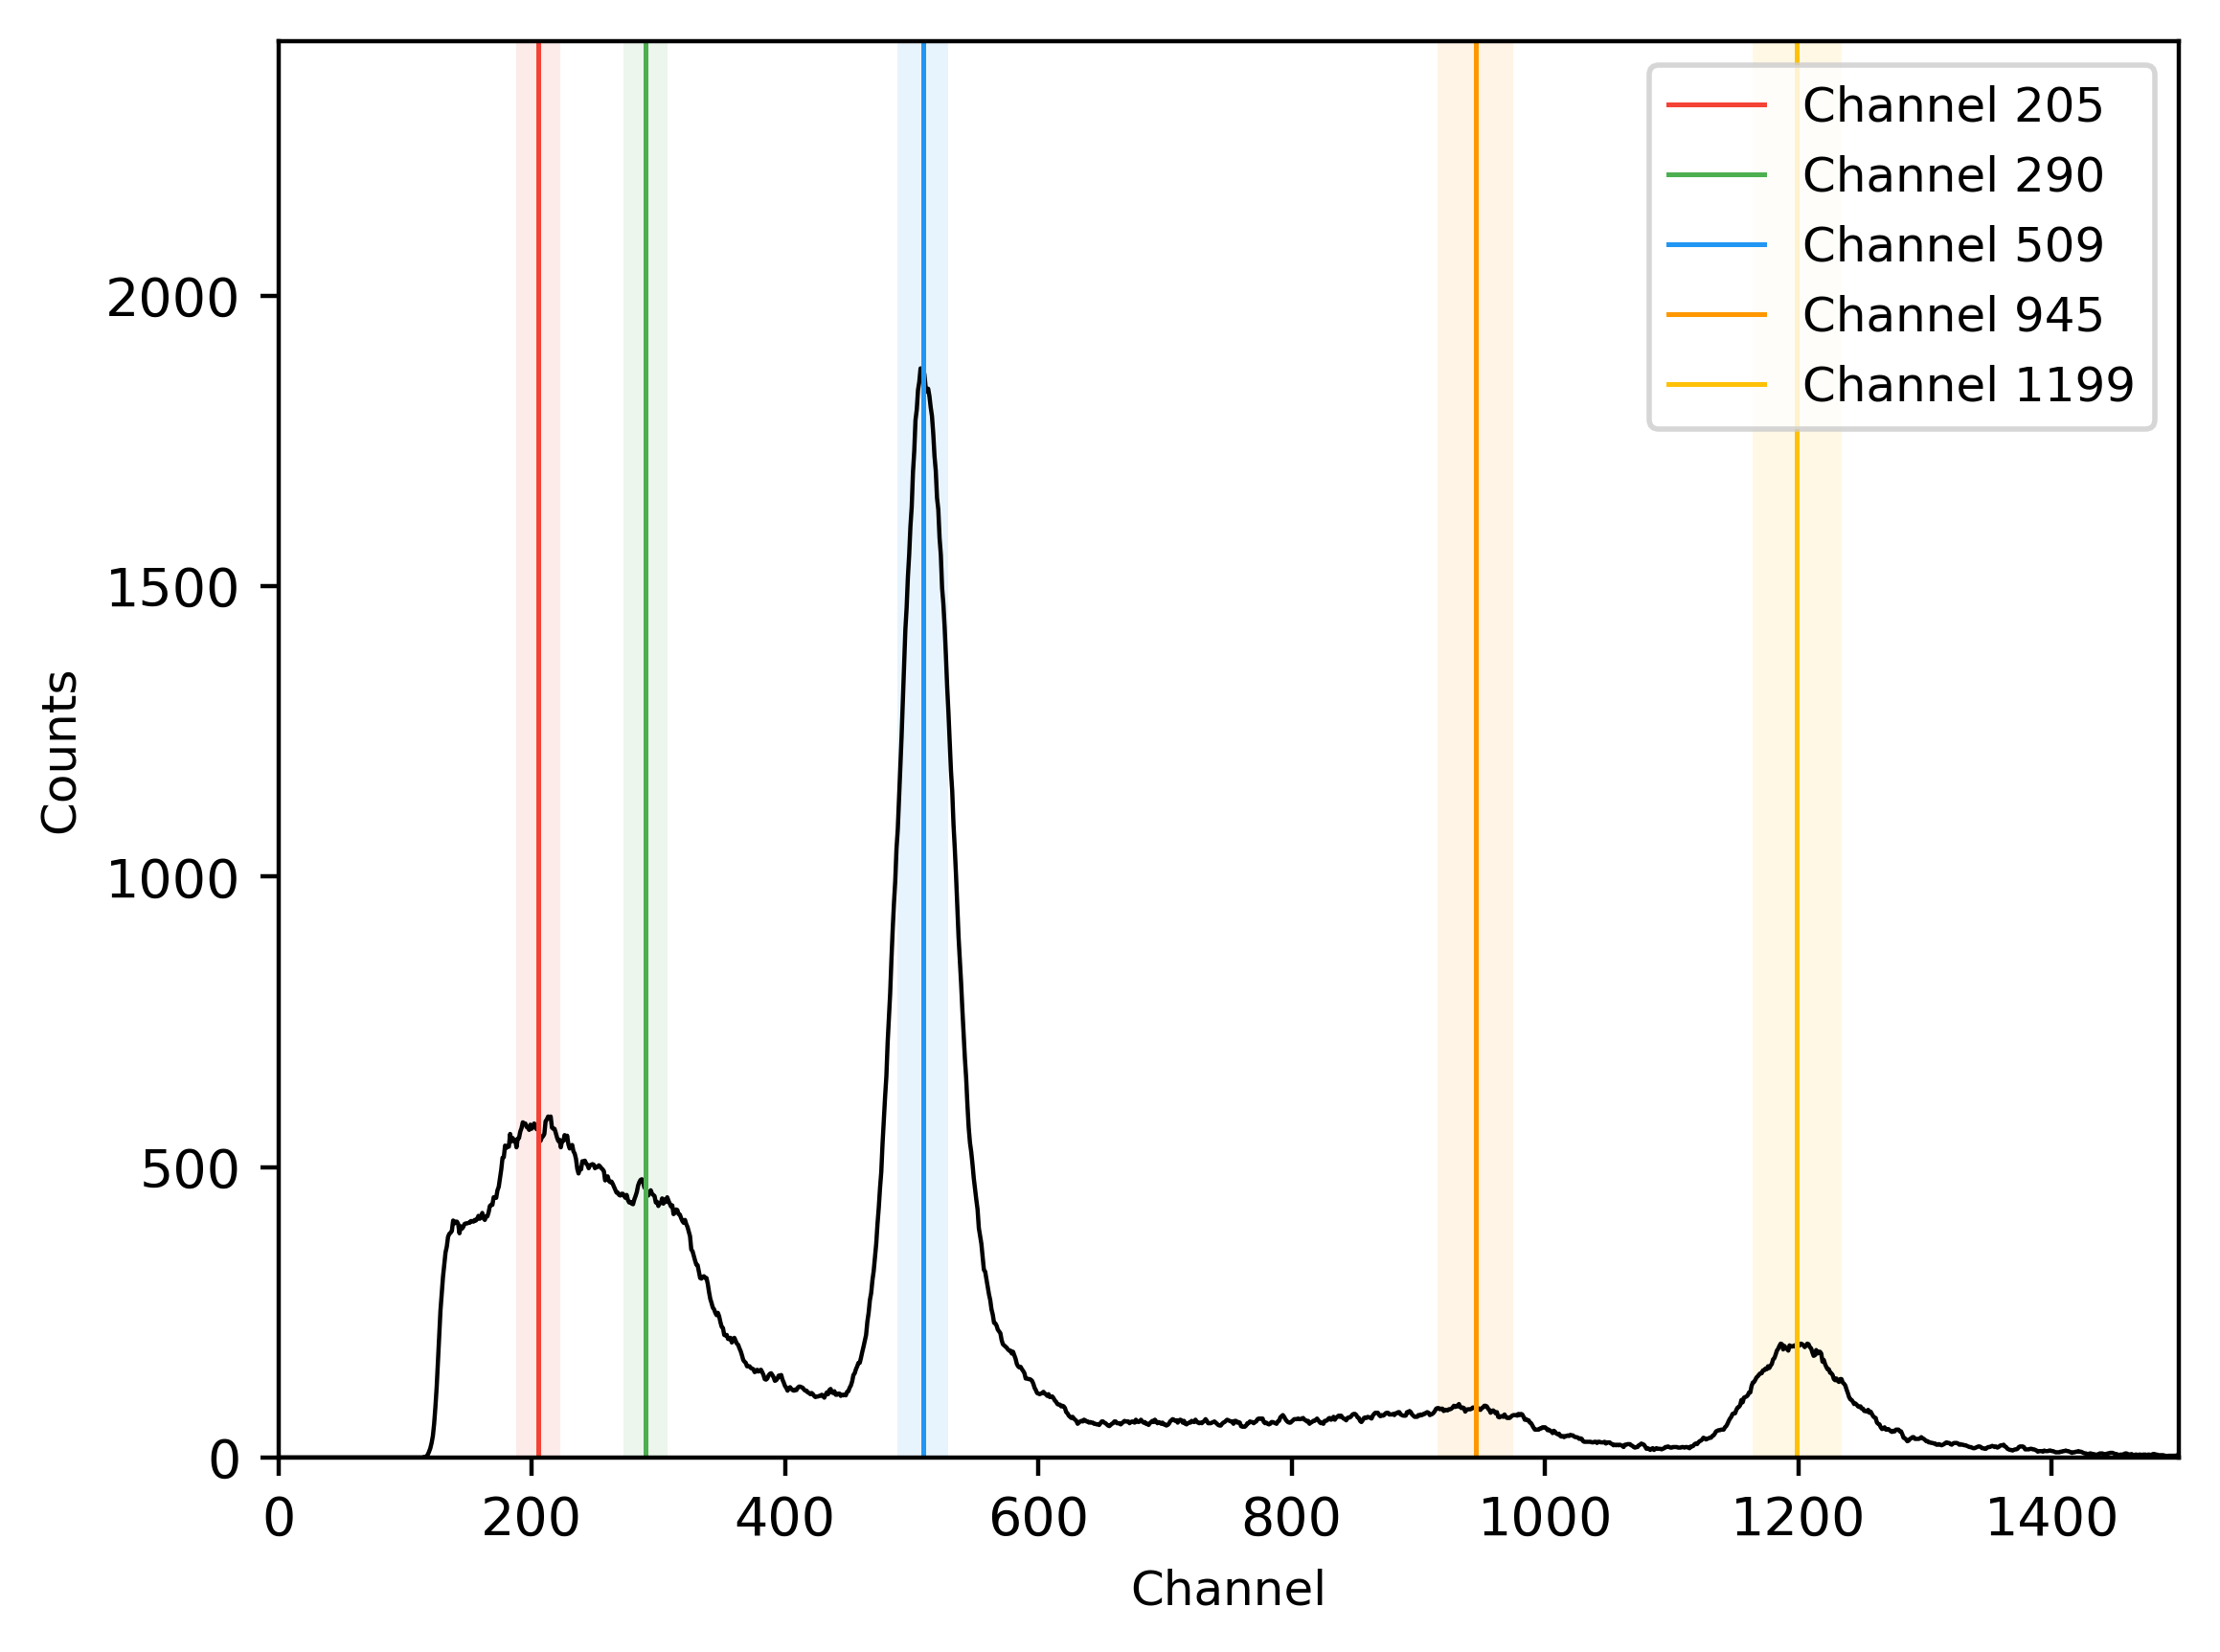
\includegraphics[width=\linewidth]{22Na}
\captionof{figure}{Decay scheme of $^{22}\text{Na}$}
\label{fig:22NaDecayScheme}
\end{multicolfloat}
%
\begin{multicolfloat}
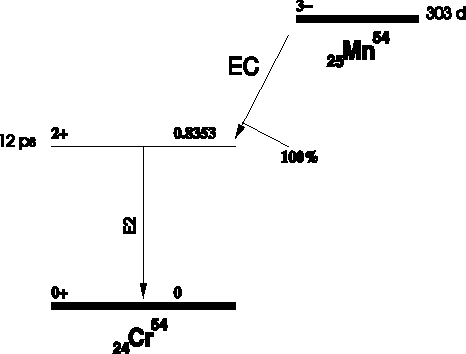
\includegraphics[width=\linewidth]{54Mn}
\captionof{figure}{Decay scheme of $^{54}\text{Mn}$}
\label{fig:54MnDecayScheme}
\end{multicolfloat}
%
\begin{multicolfloat}
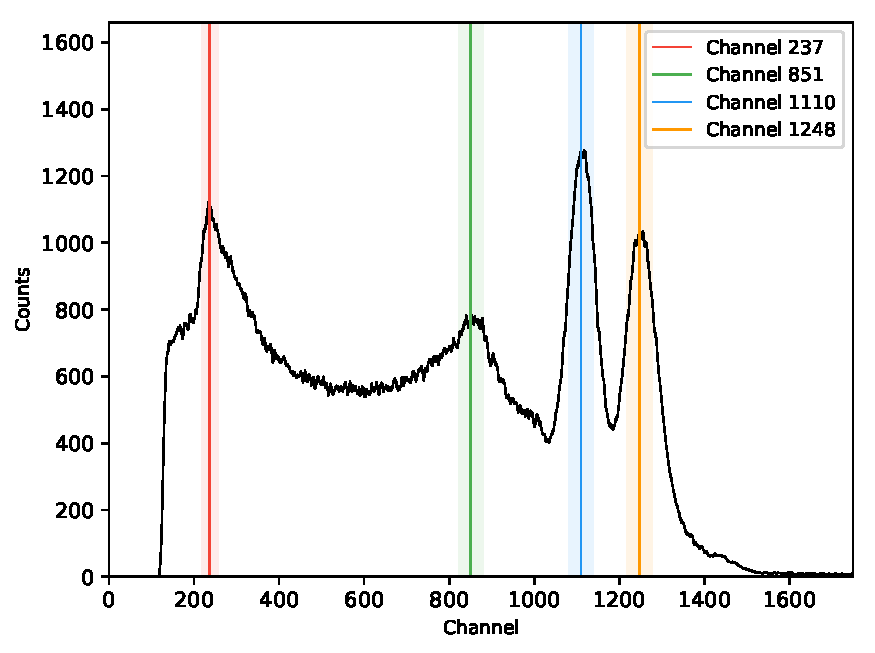
\includegraphics[width=\linewidth]{60Co}
\captionof{figure}{Decay scheme of $^{60}\text{Co}$}
\label{fig:60CoDecayScheme}
\end{multicolfloat}
%
\begin{multicolfloat}
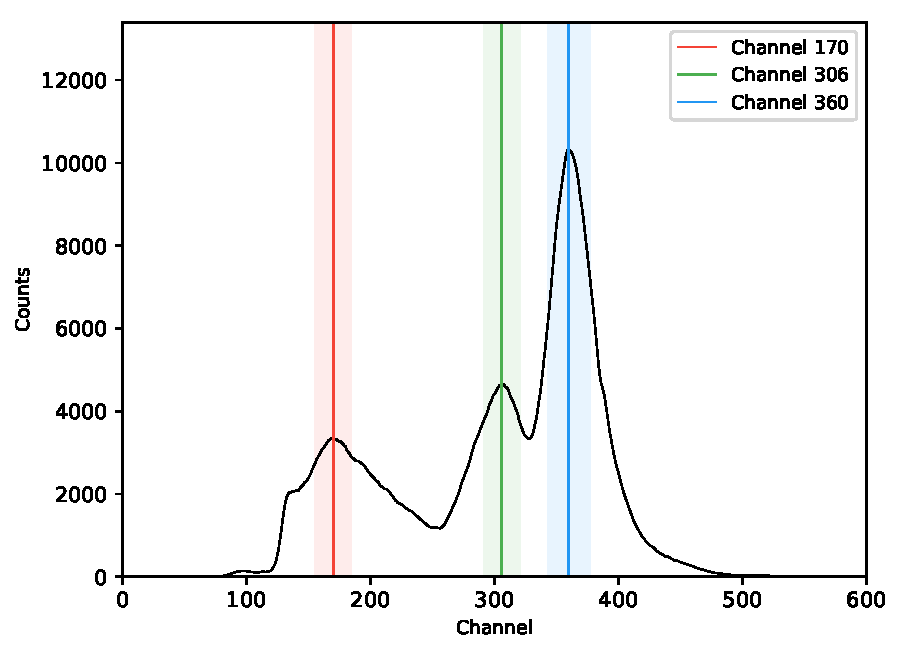
\includegraphics[width=\linewidth]{133Ba}
\captionof{figure}{Decay scheme of $^{133}\text{Ba}$}
\label{fig:133BaDecayScheme}
\end{multicolfloat}
%
\begin{multicolfloat}
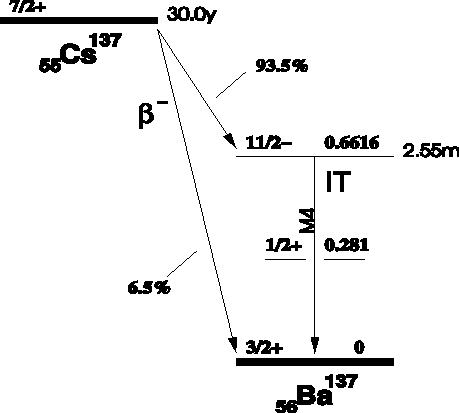
\includegraphics[width=\linewidth]{137Cs}
\captionof{figure}{Decay scheme of $^{137}\text{Cs}$}
\label{fig:137CsDecayScheme}
\end{multicolfloat}
%
\subsection{Circuit schematics}
%
\begin{multicolfloat}
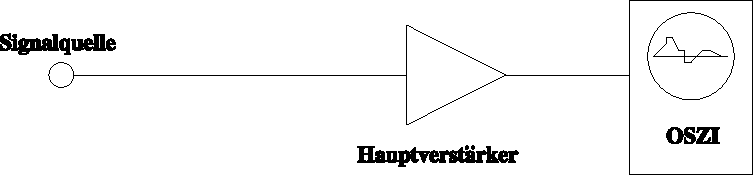
\includegraphics[width=\linewidth]{Schaltung1}
\captionof{figure}{Circuit schematic 1}
\label{fig:Schaltung1}
\end{multicolfloat}
%
\begin{multicolfloat}
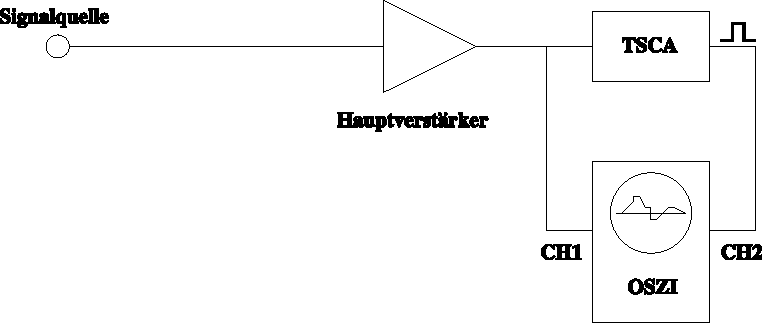
\includegraphics[width=\linewidth]{Schaltung2}
\captionof{figure}{Circuit schematic 2}
\label{fig:Schaltung2}
\end{multicolfloat}
%
\begin{multicolfloat}
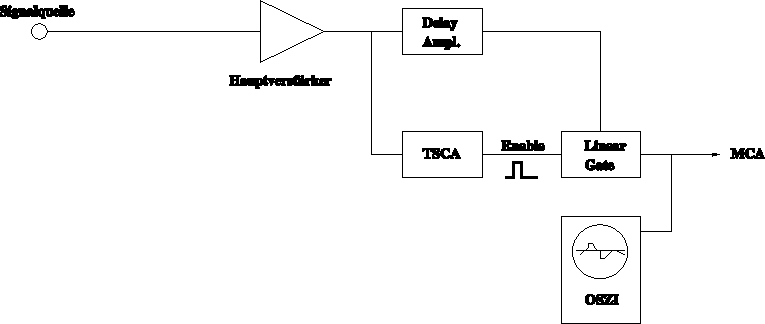
\includegraphics[width=\linewidth]{Schaltung3}
\captionof{figure}{Circuit schematic 3}
\label{fig:Schaltung3}
\end{multicolfloat}
%
\begin{multicolfloat}
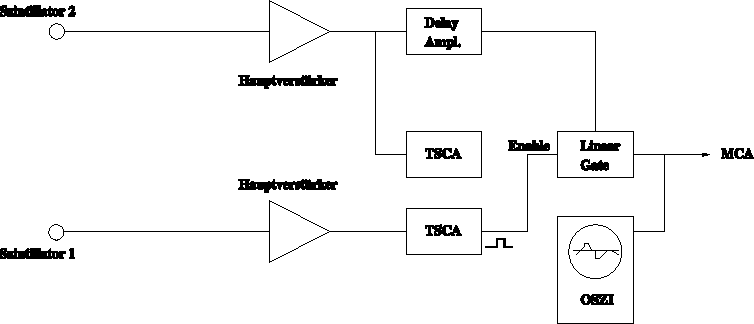
\includegraphics[width=\linewidth]{Schaltung4}
\captionof{figure}{Circuit schematic 4}
\label{fig:Schaltung4}
\end{multicolfloat}
%
\begin{multicolfloat}
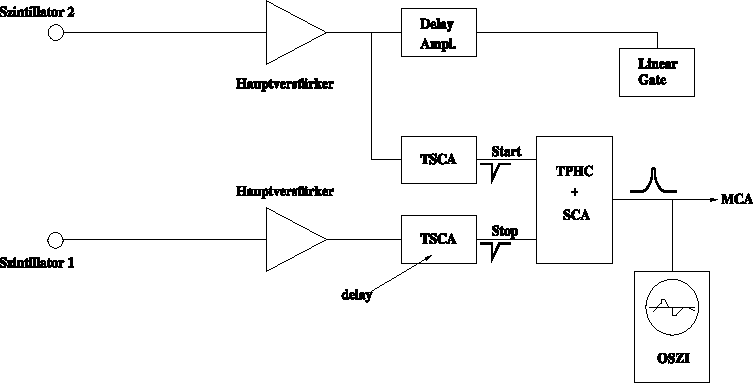
\includegraphics[width=\linewidth]{Schaltung5}
\captionof{figure}{Circuit schematic 5}
\label{fig:Schaltung5}
\end{multicolfloat}
%
\begin{multicolfloat}
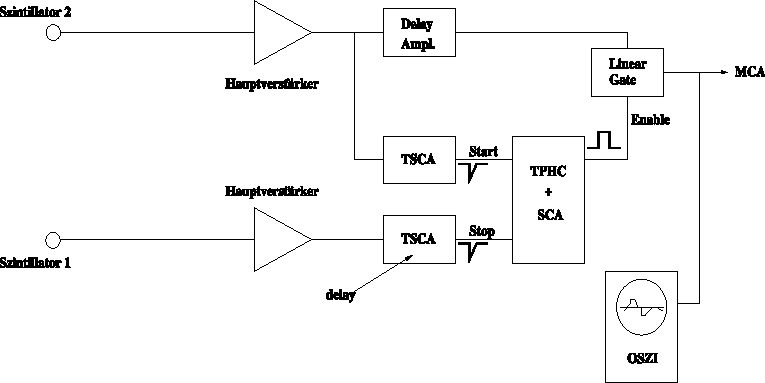
\includegraphics[width=\linewidth]{Schaltung6}
\captionof{figure}{Circuit schematic 6}
\label{fig:Schaltung6}
\end{multicolfloat}


\end{document}
